\documentclass[pdftex,11pt]{article}

\usepackage[dvips]{graphicx}            % to include images
\usepackage[portuguese]{babel}
\usepackage{setspace}
\usepackage{float}
\usepackage{amssymb}
\usepackage{amsmath}
\usepackage{cite}
\usepackage{times}
\usepackage{url}
\usepackage{listings}
\usepackage{placeins} % floatbar

%\bibliography{projeto}
\bibliographystyle{plain}
\def\refname{Referências Bibliográficas}

\oddsidemargin 0pt
\evensidemargin 0pt
\marginparwidth 0pt
\topmargin 50pt
\headheight 0pt
\headsep 0pt
%\footheight 0pt
\footskip 30pt
\textwidth 470pt
\textheight 600.5pt

\usepackage[utf8]{inputenc}

\title{Relatório PIBIC quota 2016-2017}

\begin{document}

\thispagestyle{empty}


\begin{center}
\Large
Instituto de Computação \\
Universidade Estadual de Campinas

\end{center}


\bigskip
\bigskip
\bigskip

{\LARGE
  \begin{center}
      \textbf{Caracterização de PUFs usando representações
              topológicas e entradas de alta entropia}

    \vspace{1cm}

   Relatório Final de Iniciação Científica
  \end{center}
}

\vfill


\hspace{3cm}
\begin{tabular}{rl}

	Aluno:  & Rodrigo de Castro Surita \\
    		& \emph{ra139095@fee.unicamp.br} \\
    \\

  	Orientador: & Mário Lúcio Côrtes \\
                & cortes@ic.unicamp.br \\

\end{tabular}
        \newpage

\begin{spacing}{1.5}
%\begin{spacing}{2.0}


\section*{Resumo}

\textit{Physical Unclonable Functions} (PUFs) são dispositivos capazes de explorar a variabilidade de processos de fabricação para criar funções pseudoaleatórias teoricamente únicas e não clonáveis. São geralmente utilizados em aplicações de segurança, como autenticação e geração de chaves, com vantagens teóricas sobre métodos tradicionais. Apesar das vantagens, muitos modelos de PUFs revelaram ser vulneráveis contra modelagem estatística, ataques de canal auxiliar e engenharia reversa.

Este projeto teve como objetivos encontrar representações topológicas para modelos PUFs e a partir destas obter modelos para ataques práticos de modelagem estatística e métricas para determinar se um PUF tem uma boa resistência teórica a ataques de modelagem, bem como uma análise preliminar do comportamento de PUFs para entradas de máxima entropia.

A partir dos modelos topológicos, foi possível obter um preditor para PUFs que possam ser representados na forma de um produto escalar. Este  obteve uma precisão de 96\% contra 99\% obtidos com o estado da arte para um Arbiter PUF de 128 estágios com 10.000 desafios aleatórios, mas com um custo computacional uma ordem de grandeza menor. A partir do uso de entradas de máxima entropia, foi possível obter um ganho de 82\% contra 74\% no Arbiter PUF, 75\% contra 68\% no XOR PUF e 80\% contra 73\% no Loop PUF, sendo assim, mais eficiente em cenários onde um atacante pode escolher quais desafios vai aplicar.


\section{Introdução}\label{sec:introducao}

Em processos industriais e fabricação de dispositivos, é comum encontrar variabilidade entre entre unidades produzidas. Apesar de geralmente indesejável, essa variação é aceitável dentro de uma certa tolerância. \textit{Physical Unclonable Functions} (PUFs) ou Funções Físicas Não Clonáveis, em tradução livre, são dispositivos que exploram estas variações estatísticas de processos de fabricação para gerar funções capazes de mapear um conjunto de entradas (ou desafios) em um conjunto de saídas (ou respostas)~\cite{bookspringerlink:10.1007} para fins de autenticação. Idealmente, diversas funções, ou instâncias, produzidas por um mesmo processo são diferentes e independentes. A relação entre desafios e respostas deve-se exclusivamente a variações aleatórias de processo. Diversos características físicas podem ser usadas para formar uma PUF, como reflexão de luz, capacitâncias, dissipação de calor, atrasos de propagação em linhas, dentre outras~\cite{bookspringerlink:10.1007,RF-DNA}. Ainda assim, tecnologias baseadas em silício tem maior relevância devido à maturidade dos processos de fabricação, facilidade de integração com sistemas digitais e uma moderada proteção contra ataques físicos~\cite{MajzoobiKP09,RfidPUF}.

PUFs possuem aplicações na área de segurança, como autenticação de dispositivos~\cite{SuhDevadas2007}, geração de chaves~\cite{LeeLGSDD_PUFSecretKey_VLSI04} e ativação remota~\cite{GassendCDD_CCSC02}. Teoricamente possuem várias vantagens sobre técnicas de autenticação tradicionais como chaves armazenadas em memórias, podendo resultar em circuitos pequenos, de baixo custo e mais resilientes à ataques.

Apesar de promissores, diversos modelos de PUFs sofreram críticas devido a vulnerabilidades presentes em algumas arquiteturas~\cite{PUFAnalysis, MajzoobiKP09, MajzoobiKP08}, que permitem ataques como:
(1) modelagem estatística e por aprendizado de máquina, usando correlações entre entradas e saídas para fins de regressão;
(2) engenharia reversa dos parâmetros aleatórios, caso os parâmetros sejam direta ou indiretamente observáveis;
(3) \textit{side-channel attacks} ou ataques de canais auxiliares, que são relacionados a vazamentos de informação não relacionados às saídas, variações no campo magnético próximo, na tensão da fonte de alimentação ou no perfil de emissão de fótons.

A sucessibilidade a modelagem estatística pode restringir o uso da função em algumas aplicações, já que pode ser realizada apenas interceptando ou enviando um conjunto de pares desafio-resposta sem que o atacante tenha acesso físico à PUF\@.
Nestes ataques, consideram-se cenários onde pressupõe-se que um atacante obteve um conjunto de pares desafio-resposta, denominado conjunto de treinamento, e a partir deste pode formar modelos de regressão e prever a resposta da função para uma novo conjunto de entradas desconhecidas~\cite{RuhrmairD13,RuhrmairSSDDS10}.

Ainda assim, novas propostas de PUFs são publicadas sem que exista uma métrica de projeto que permita estimar se um projeto terá uma resistência esperada a ataques de modelagem, sendo que só é possível determinar estas propriedades aplicando diversos métodos de aprendizado sobre implementações dos dispositivos e verificando se a precisão dos modelos está dentro de valores esperados. Também não existem modelos de aprendizado que são comprovadamente eficientes em subclasses de PUFs, sendo que é necessário verificar o melhor modelo por tentativa e erro.


\section{Trabalhos Relacionados}\label{sec:relacionados}


    Uma propriedade frequentemente explorada para construção de PUFs é o atraso de propagação em ligações elétricas de circuitos integrados. Estes são batizados de PUFs baseados em atraso ou \textit{delay PUFs}\cite{bookspringerlink:10.1007}. Uma das primeiras arquiteturas publicadas usando esta característica, que motivou diversas outras, é batizada de \textit{Arbiter PUF}~\cite{GassendLCDD04}. Este modelo depende de dois pulsos elétricos chaveados por uma série de $N$ CrossBars (Figura~\ref{fig:apuf}). Uma entrada binária (ou desafio) é aplicada de forma que cada bit chaveia um crossBar (Figura~\ref{fig:crossbar}). Como os atrasos entre as trilhas diferem entre si, os pulsos terminam a série com uma certa defasagem que difere entre os dois estados do crossBar e consequentemente entre desafios escolhidos. Para medir a defasagem é colocado um árbitro, implementado com um Flip-Flop D alimentado pelas linhas nas entradas D e Clk. A resposta do árbitro será 1 caso o sinal D seja mais rápido e 0 caso contrário.


\begin{figure}
\centering
\label{fig:crossbar}
\includegraphics[width=4cm]{crossbar.png}
\caption{Crossbar Implementado com dois multiplexadores.}
\end{figure}


\begin{figure}
\label{fig:apuf}
\centering
\includegraphics[width=10cm]{apuf.png}
\caption{Representação de um Arbiter PUF com N níveis.}
\end{figure}


Em cada crossBar existem 4 parâmetros aleatórios de processo considerados, referentes ao atraso de cada uma das possíveis linhas (Equações~\ref{eq:crossbar} e~\ref{eq:crossba2}), porém para a estimativa da diferença entre pulsos são relevantes apenas as diferenças entre canais opostos do crossBar. Sendo assim, cada crossBar possuí apenas 2 parâmetros aleatórios independentes.

\begin{eqnarray}
\label{eq:crossbar}
Q_1 = \left\{
	\begin{array}{ll}
		X_1 \ \mbox{after } \ d_1  & \mbox{if } c = 0 \\
		X_2 \ \mbox{after } \ d_2  & \mbox{if } c = 1
	\end{array}
\right.
\end{eqnarray}

\begin{eqnarray}
\label{eq:crossba2}
Q_2 = \left\{
	\begin{array}{ll}
		X_2 \ \mbox{after } \ d_3  & \mbox{if } c = 0 \\
		X_1 \ \mbox{after } \ d_4  & \mbox{if } c = 1
	\end{array}
\right.
\end{eqnarray}


Quando crossBars são agrupados em um APUF de N estágios, é possível ainda representá-lo pelo seu Modelo Linear Aditivo~\cite{ArbiterPUF-master-thesis}, no qual são consideradas apenas $N+1$ variáveis e na qual a resposta da função $y$ é dada pelo sinal de uma operação de produto interno. Está representação é obtida aplicando uma transformação de paridade sobre o vetor de entrada $C$, cujo resultado é denominado $P$, e uma soma das diferenças dos sinais dos $N$ estágios, denotada $W$.

$$\ y = sign( \vec{W} \cdot \vec{P} ) $$


A seguir são dadas as expressões para $p_k$ e $w_k$, sendo o k-ésimo elemento dos vetores $P$ e $W$.

$$ p_k = \prod_{i=k+1}^{n} c_i$$

$$ \alpha_k = \frac{d_{1k} - d_{2k} + d_{3k} - d_{4k}}{2} $$
$$ \beta_k  = \frac{d_{1k} - d_{2k} - d_{3k} + d_{4k}}{2} $$
$$ w_k = \alpha_k + \beta_{k-1} $$


O XOR PUF\cite{SuhDevadas2007} é uma variante do Arbiter PUF criada para fins de melhorar vulnerabilidades de seu predecessor na qual um conjunto de linhas de Arbiter PUF e exercitada em paralelo, e a resposta do sistema é dada pela operação de ou-exclusivo entre os resultados de cada linha.

\begin{figure}
\label{fig:xorpuf}
\centering
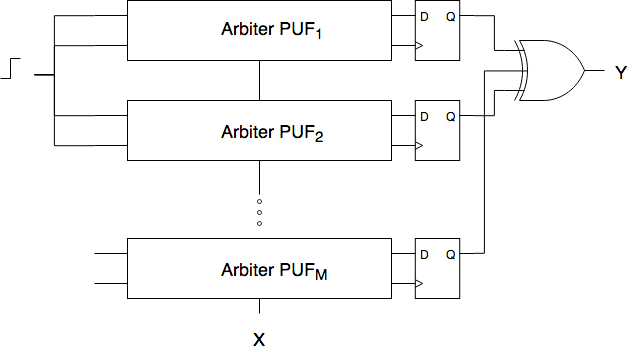
\includegraphics[width=10cm]{xorpuf.png}
\caption{XOR PUF agregando M Arbiter PUFs com N níveis.}
\end{figure}

Tanto para o Arbiter PUF como para o XOR PUF existem algumas publicações sobre ataques de aprendizado de máquina bem sucedidos~\cite{RuhrmairD13, RuhrmairSSDDS10}. Usando regressões logísticas, são atingidas precisões acima de $99\%$ com um número de pares desafio-resposta de treinamento na escala entre $10^4$ e $10^6$.

O Loop PUF\cite{looppuf} é outra arquitetura baseada em atrasos onde um sinal atravessa uma série de multiplexadores e acumula atrasos de apenas um dos caminhos, selecionado pelo desafio. Ao contrário do Arbiter PUF, o loop PUF não cruza sinais em cada nível. Um sinal de entrada pode ser mantido em um loop astável por um período definido de tempo e a resposta pode ser dada comparando a frequência de oscilação com um conjunto de desafios ou uma constante de referência. Cada multiplexador contribui com um parâmetro aleatório correspondendo a diferença entre os dois caminhos.

\begin{figure}
\label{fig:apuf}
\centering
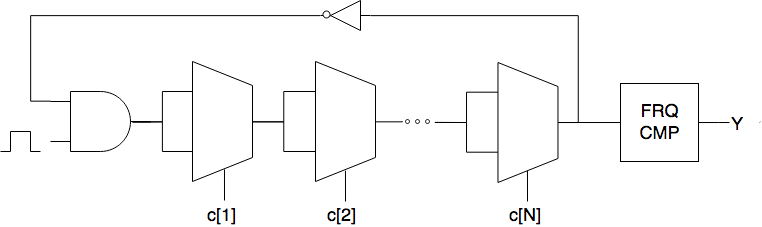
\includegraphics[width=10cm]{looppuf.png}
\caption{Loop PUF com N níveis.}
\end{figure}

Para um Loop PUF, não existem resultados publicados sobre a resistência a ataques por aprendizado de máquina. No entanto, este possui um resultado publicado para o código de maximiza a entropia da entrada~\cite{hadamard}, ou seja, o número de caminhos percorridos, dado um limite de entradas. Este resultado depende apenas das hipóteses de que a distribuição de parâmetros é gaussiana e que o resultado do PUF pode ser descrito por um produto interno. porém não foram resultados semelhantes para outras arquiteturas. Nesta arquitetura, o código de máxima entropia
são matrizes de hadamard~\cite{hadamard} com um número de colunas compatível ao número de entradas do PUF.

%Conforme descrito nas equações~\ref{eq:crossbar} e~\ref{eq:crossba2}, o Arbiter
%PUF representa uma função binária que satisfaz as condições para os espaços propostos
%com dimensão $N = M+1$, sendo $M$ o número de CrossBars do PUF\@.

\section{Metodologia}\label{sec:atividades}


\subsection{Soluções em espaços N-dimensionais}

Este trabalho propôs como algumas hipóteses para modelar um PUF representado por meio do modelo linear aditivo como uma função do tipo do tipo $f: \mathbb{B}^n \to \mathbb{B}$ usando as seguintes abordagens.


\subsubsection{Representação em parâmetros aleatórios}\label{sec:polytope}

Consideramos que cada instãncia de PUF representa um ponto em um espaço de
dimensão equivalente ao número de parâmetros $N$ e cuja a posição
é definida pelo valor em que cada parâmetro aleatório assume em cada instância, e que
cada desafio representa uma curva de dimensão $N-1$ (ou uma desigualdade) que divide
o espaço em dois. Neste espaço, uma PUF na forma de seu modelo linear aditivo possuí
as seguintes propriedades:


\begin{spacing}{1.0}
\begin{enumerate}
\item Cada desafio representa um hiperplano.
\item Todos os hiperplanos (desafios) passam pela origem.
\item Um PUF está sempre contido no volume definido pela intersecção de seus desafios.
\end{enumerate}
\end{spacing}


No entanto, em etapas subsequentes do projeto, a representação originalmente proposta
se mostrou impraticável em termos de complexidade matemática, sendo assim, uma nova
representação foi proposta.

\subsubsection{Representação por classificação de entradas}\label{sec:hypercube}

Cada desafio representa um vértice de um hipercubo
de dimensão equivalente ao número de entradas binárias $N$, e cada  instancância
de PUF representanta
uma curva (ou desigualdade) de dimensão $N-1$. que divide o espaço em duas classes.
Neste espaço outro, destacam-se as seguintes características:


\begin{spacing}{1.0}
\begin{enumerate}
\item Representa um conjunto linearmente separável, ou seja, a instância de PUF é descrita apenas por um hiperplano que divide os vértices correspondentes as saídas.
\item Todos os hiperplanos (PUFs) passam pela origem.
\item Todos os hiperplanos (PUFs) dividem os vértices em duas metades com o mesmo número de vértices.
\item Para cada PUF, um desafio sempre está na classe oposta ao seu inverso ou dual.
\end{enumerate}
\end{spacing}


\subsection{Heurísticas de modelagem}


\subsubsection{Aproximação por volume}

Uma das propostas de heurísticas de modelagem baseou-se na hipótese de que dentro do
no espaço de solução em parâmetros aleatórios definido em~\ref{sec:polytope},
seria possível obter um cone a partir de um conjunto de desafios e estimar para um dado PUF
a probabilidade de ele estar dentro deste cone por uma medida de volume de uma extensão
limitada do mesmo.

\subsubsection{Aproximação por vetor normal}

Uma outra proposta muito simples baseada nas propriedades definidas em~\ref{sec:hypercube},
parte do princípio de que o vetor normal ao hiperplano de um Arbiter PUF sobre o hipercubo
de entradas tem a mesma direção da soma dos vetores que ligam a origem aos desafios
de um dos lados do hiperplano. A hipótese é que se consideramos um subconjunto grande
de desafios conhecidos, a soma dos vetores entre a origem e os vértices conhecidos
de um lado do hiperplano deve aproximar o vetor normal do PUF que a ser modelado,
e pode ser usado como preditor.
Se consideramos também a propriedade (4), também podemos considerar os vetores duais
da região contrária.

\subsection{Soluções por aprendizado de máquina usando entradas de máxima entropia}

Nesta outra abordagem, parte-se do princípio que melhorar os algoritmos usados no estado da arte como preditores para PUFs teria pouco efeito, já que os mesmos são utilizados em diversas outras aplicações e que são comprovadamente aproximadores universais para problemas linearmente separáveis~\cite{WESTREICH2010826}. Ao contrário das outras abordagens, esta propõe melhorar o desempenho das técnicas utilizadas na literatura escolhendo códigos de entrada que permitam aprender mais rapidamente instâncias de PUFs ao invés de usar entradas aleatórias. Para este fim, destaca-se o uso do código de máxima entropia publicado para o Loop PUF. A hipótese é que uma vez que códigos de maior entropia permitem caracterizar mais rapidamente uma função, também serviriam para um algoritmo de aprendizado de máquina reproduzi-la com maior precisão.

Dadas as hipóteses usadas para derivar o resultado para o Loop PUF, também podem ser estendidos resultados para outras PUFs que possam ser representadas por meio de um produto escalar, ou seja, que possuam um modelo linear aditivo, como o Arbiter PUF e o XOR PUF. Para obter os códigos para tais funções, bastaria aplicar a antitransformada sobre o vetor para obter o código que deveria ser aplicado nas entradas da PUF.


\section{Resultados}\label{sec:resultados}

As propostas apresentadas na metodologia foram testadas usando simulações de Monte Carlo sobre implementações digitais dos circuitos implementadas usando linguagem Python e a biblioteca freePUF \cite{freepuf}. Detalhes de cada experimento são apresentados nas respectivas seções.

\subsection{Aproximação por volume}

Esta abordagem obteve bons resultados em implementações
com dimensão reduzida de Arbiter PUFs, mas se mostrou impraticável
em modelos de dimensões propostas para aplicações.

Também foram explorados métodos aproximados de cálculo de volume \cite{Enge1998ExactVC},
mas que não tiveram bons resultados, seja por que a aproximação seria
imprecisa ou porque a hipótese esta incorreta, ainda que não haja uma
contraprova para a mesma.

\subsection{Aproximação por vetor normal}

 Os resultados para o preditor por aproximação por vetor normal demonstraram ser um
pouco piores em precisão que os estado da arte usado para predizer PUFs,
porém possuem um custo computacional uma ordem de grandeza inferior.

\begin{table}[H]
\centering
\caption{Resultados preliminares para o preditor por aproximação normal para uma média de 1.000 Arbiter PUF de 128 CrossBars com 10.000 desafios.}
\label{normal-pred}
\begin{tabular}{|l|l|l|}
\hline
Técnica             & Precisão (\%) & Tempo de CPU (s) \\ \hline
SVM linear          & 99.2          & 2.902            \\ \hline
Regressão logística & 99.0          & 2.180            \\ \hline
Aproximação normal  & 95.6          & 0.168            \\ \hline
\end{tabular}
\end{table}


\subsection{Aprendizado de máquina usando entradas de máxima entropia}

Nesta abordagem, foram inicialmente obtidos os códigos de máxima entropia para o Arbiter PUF e o XOR PUF a partir do código publicado para o Loop PUF. Os códigos foram computados por meio da antitransformada do modelo linear aditivos aplicada sobre a matriz de Hadamard usada para o Loop PUF. Para o caso de um Arbiter PUF de 8 estágios, a matriz resultante é apresentada abaixo.


\[
\begin{bmatrix}
    +1 & +1 & +1 & +1 & +1 & +1 & +1 & +1 \\
    -1 & -1 & -1 & -1 & -1 & -1 & -1 & -1 \\
    +1 & -1 & +1 & -1 & +1 & -1 & +1 & -1 \\
    -1 & +1 & -1 & +1 & -1 & +1 & -1 & +1 \\
    +1 & +1 & +1 & -1 & +1 & +1 & +1 & -1 \\
    -1 & -1 & -1 & +1 & -1 & -1 & -1 & +1 \\
    +1 & -1 & +1 & +1 & +1 & -1 & +1 & +1 \\
    -1 & +1 & -1 & -1 & -1 & +1 & -1 & -1
\end{bmatrix}
\]

Para os experimentos de aprendizado de máquina, foram usadas SVMs e regressões logísticas. Os resultados são amplamente comparáveis, então são apresentados apenas os resultados para SVMs.

São apresentadas nas figuras \ref{fig:ml-hadamard-apuf}, \ref{fig:ml-hadamard-xorpuf} e \ref{fig:ml-hadamard-looppuf} a precisão dos algoritmos de aprendizado de máquina para uma média de 1.000 instancias de Arbiter PUF, XOR PUF e Loop PUF de 1024 estágios verificadas sobre um conjunto de 10.000 desafios de teste. A precisão para o Arbiter PUF e o XOR PUF com entradas aleatórias é comparável com resultados publicados na literatura. Para o Loop PUF, não são conhecidos resultados para aprendizado de máquina na literatura, mas experimentos mostraram que este tem uma imprevisibilidade muito próxima a do Arbiter PUF.

\begin{figure}
\label{fig:ml-hadamard-apuf}
\centering
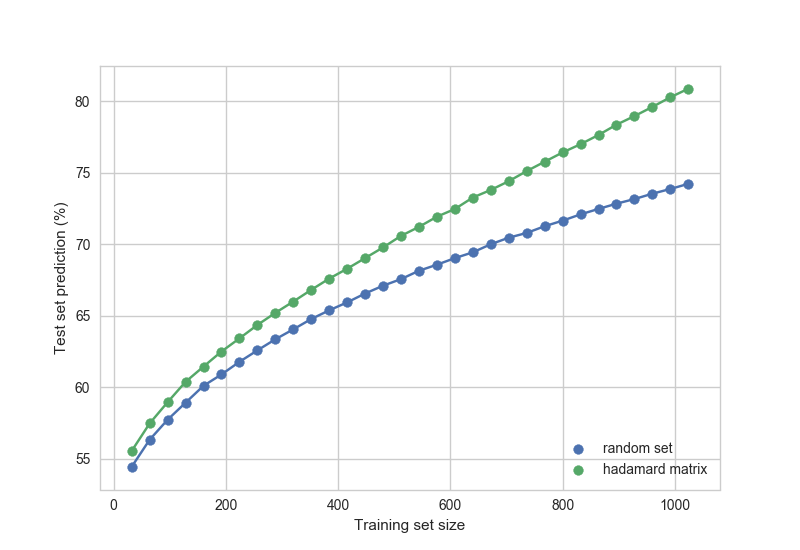
\includegraphics[width=12cm]{ml-hadamard-apuf.png}
    \caption{Precisão para o conjunto de testes em relação ao tamanho do conjunto de treinamento para uma média de 1000 Arbiter PUF de 1024 estágios usando códigos de alta entropia e entradas aleatórias.}
\end{figure}

\begin{figure}
\label{fig:ml-hadamard-xorpuf}
\centering
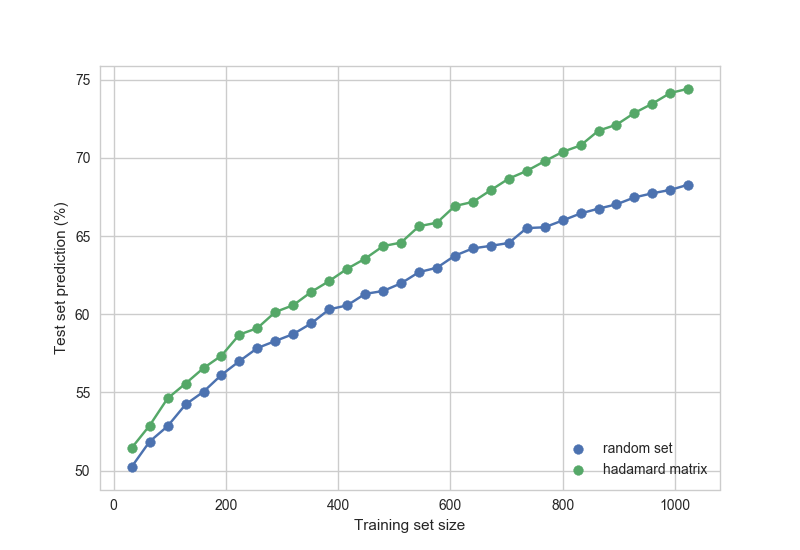
\includegraphics[width=12cm]{ml-hadamard-xorpuf.png}
\caption{Precisão sobre um conjunto de testes de 10.000 desafios em relação ao tamanho do conjunto de treinamento para uma média de 1000 XOR PUF de 1024 estágios com duas linhas usando códigos de alta entropia e entradas aleatórias.}
\end{figure}


\begin{figure}
\label{fig:ml-hadamard-looppuf}
\centering
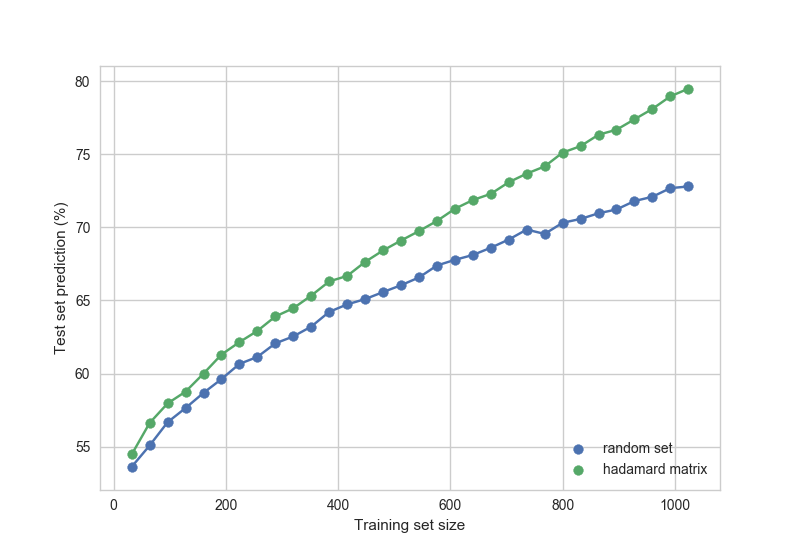
\includegraphics[width=12cm]{ml-hadamard-looppuf.png}
\caption{Precisão sobre um conjunto de testes de 10.000 desafios em relação ao tamanho do conjunto de treinamento para uma média de 1000 Loop PUF de 1024 estágios usando códigos de alta entropia e entradas aleatórias.}
\end{figure}


Nota-se que as taxas de aprendizado para entradas de alta entropia são consideravelmente mais altas, atingindo 82\% contra 74\% no Arbiter PUF,  75\% contra 68\% no XOR PUF e 80\% contra 73\% no Loop PUF.

Na figura \ref{fig:ml-cmp-apuf} são apresentados resultados variando o tamanho do Arbiter PUF e do desafio de treinamento para entradas aleatórias e para entradas de alta entropia. Vale notar que enquanto que a relação entre precisão e tamanho da entrada cai para entradas aleatórias, a mesma permanece quase constante para entradas de alta entropia. Isto representa um indicio que aumentar o número de estágios na PUF aumenta apenas linearmente a dificuldade de aprendê-la usando códigos de alta entropia.

\begin{figure}[H]
\label{fig:ml-cmp-apuf}
\centering
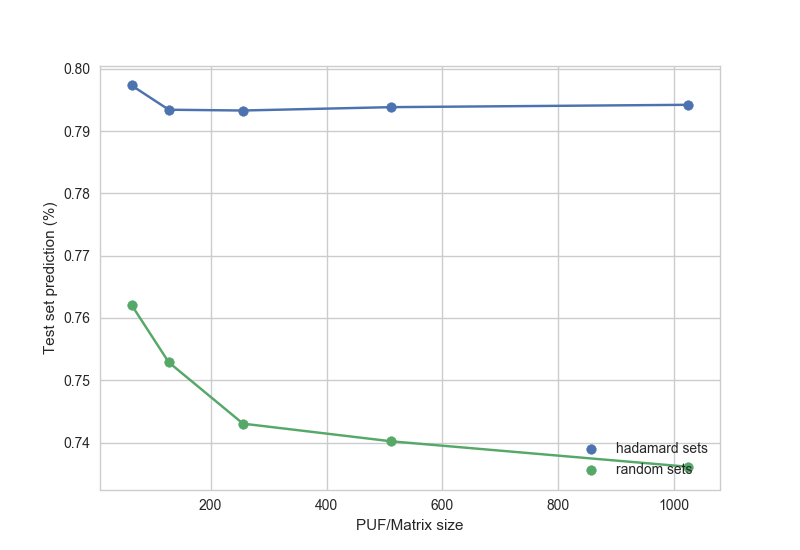
\includegraphics[width=12cm]{ml-cmp-apuf.png}
\caption{Precisão sobre um conjunto de testes de 10.000 desafios para um conjunto de treinamento de tamanho $N$ em para uma média de 1.000 Arbiter PUF de $N$ estágios usando códigos de alta entropia e entradas aleatórias em função de $N$.}
\end{figure}

\section{Conclusões}\label{sec:conclusoes}

Este trabalho investigou fundamentalmente duas abordagens para caracterizar e modelar PUFs, sendo uma baseada no estudo de novas técnicas baseadas na representação da função em espaços N-dimensionais e outra baseada em técnicas de aprendizado de máquina convencionais, mas com uso de entradas de máxima entropia.

Para a abordagem em espaços n-dimensionais, foram consideradas duas representações, sobre as quais foram obtidas duas heurísticas de solução. A primeira representa uma instância de PUF como um ponto em um espaço de N parâmetros aleatórios e um desafio como um hiperplano de tamanho N-1 que dividia o espaço ao meio. Sobre este modelo foi derivada uma aproximação por meio do volume ocupado delimitado por um conjunto de desafios, que se mostrou possível para instâncias pequenas, mas inviável computacionalmente para instâncias grandes. Outras abordagens usando esta representação podem ser viáveis, mas nota-se que como se trata de um espaço mal delimitado em $R^N$, é pouco provável que seja possível obter heurísticas que sejam ao mesmo tempo menos custosas e mais eficientes que métodos de aprendizado de máquina.

Uma segunda representação foi obtida a considerando cada desafio como um vértice de um hipercubo e cada instância de PUF como um hiperplano que divide o hipercubo em dois. Sobre esta foi derivada uma heurística que aproxima o vetor normal ao hiperplano da instância pela soma dos vetores formados pela origem e vértices representando desafios cuja resposta é conhecida. Este preditor obteve bons resultados um pouco abaixo do estado da arte na modelagem de PUFs com um custo computacional cerca de uma ordem de grandeza menor. Novas formas de aprimorar este preditor são possíveis na medida que na implementação este usou apenas uma operação simples de soma vetorial.

Apesar do resultado positivo para o preditor sobre o hipercubo, houve consenso entre os autores que talvez tentar superar a precisão dos algoritmos de aprendizado de máquina para o problema fosse pouco efetivo, e que talvez fosse mais efetivo investigar como melhorar o desempenho investigando as entradas aplicadas sobre o aprendizado. Sobre um resultado para publicado para o Loop PUF, foi possível estender códigos de alta entropia para arquiteturas como o Arbiter PUF e o XOR PUF, para as quais são publicados resultados de precisão para algoritmos de aprendizado de máquina na literatura.

O trabalho foi capaz de incluir resultados de aprendizado de máquina com entradas aleatórias para o Loop PUF e reproduzir os resultados da literatura para o Arbiter PUF e XOR PUF, no mais, o uso de entradas de alta entropia mostrou aumentar consideravelmente a precisão dos algoritmos. Sendo encorajada em cenários onde um atacante pode escolher quais desafios que aplicar. Além disso, vale ressaltar que uma investigação do comportamento linear para o aprendizado usando códigos de alta entropia pode desencorajar propostas que possam ser representadas na forma de um produto vetorial que tenham dimensão comparável à quantidade de hardware.

Como proposta de trabalhos futuros, destaca-se um estudo mais detalhado sobre o comportamento de códigos de alta entropia sobre outras métricas, como a entropia da saída, e a extensão do código para saídas maiores que $N$.


\section{Produção científica}\label{sec:producao}

Este trabalho ainda não gerou produção científica, mas representa uma extensão de um trabalho publicado pelo aluno e o orientador~\cite{7723585}. Outro artigo sobre o impacto do uso de códigos de alta entropia está previsto como extensão deste trabalho.

\section{Agradecimentos}\label{sec:agradecimentos}

Agradecemos ao CNPq e a Unicamp pelo fomento via bolsa PIBIC nos primeiros meses do projeto.


\def\refname{Referências Bibliográficas}
\bibliography{pufbib}

\end{document}
